\documentclass[../main.tex]{subfiles}
\begin{document}

\ifSubfilesClassLoaded{
	\mainmatter
	\setcounter{chapter}{6}
	\setcounter{section}{1}
}{}

\section{Charmonium Cross Section}

\subsection{Massfit results}
Like the Drell-Yan analysis, the two data sets are analyzed separately.
Using the fact that $J/\psi$ and $\psi'$ are mass resonances and correspond to peaks in the mass spectrum,
the kinematic distributions are extracted from mass decompositions performed independently in each kinematic bins.
The fits in the first $x_F$ bin is shown in \cref{fig:massfit_1st_xF},
and the fits in the other $x_F$ bins are shown in \cref{M-sec:a3_xFbin}.
The data in each bin is very well described by the fitting procedure.
The $J/\psi$ and $\psi'$ yields can then be extracted from the fits directly.

\begin{figure}[h!]
	\centering
	\begin{subfigure}{0.48\linewidth}
		\includegraphics[width=\linewidth]{massfit/run2-3/LH2/xF/LH2_xFbin0}
	\end{subfigure}
	\begin{subfigure}{0.48\linewidth}
		\includegraphics[width=\linewidth]{massfit/run2-3/LD2/xF/LD2_xFbin0}
	\end{subfigure}
	\begin{subfigure}{0.48\linewidth}
		\includegraphics[width=\linewidth]{massfit/run5-6/LH2/xF/LH2_xFbin0}
	\end{subfigure}
	\begin{subfigure}{0.48\linewidth}
		\includegraphics[width=\linewidth]{massfit/run5-6/LD2/xF/LD2_xFbin0}
	\end{subfigure}
	\caption{Mass fit for the first $x_F$ bin ($0.5\leq x_F<0.6$) for both \ce{LH_2} (left) and \ce{LD_2} (right) targets
		and both run 2-3 (top) and run 5-6 (bottom). }
	\label{fig:massfit_1st_xF}
\end{figure}
Similarly, the $P_T$ distributions are extracted from the individual fits in $P_T$ bins.
The fits for the first $P_T$ bin are shown in \cref{fig:massfit_1st_pT},
and the fits for the other bins are shown in \cref{M-sec:a3_pTbin}.
\begin{figure}[h!]
	\centering
	\begin{subfigure}{0.48\linewidth}
		\includegraphics[width=\linewidth]{massfit/run2-3/LH2/pT/LH2_pTbin0}
	\end{subfigure}
	\begin{subfigure}{0.48\linewidth}
		\includegraphics[width=\linewidth]{massfit/run2-3/LD2/pT/LD2_pTbin0}
	\end{subfigure}
	\begin{subfigure}{0.48\linewidth}
		\includegraphics[width=\linewidth]{massfit/run5-6/LH2/pT/LH2_pTbin0}
	\end{subfigure}
	\begin{subfigure}{0.48\linewidth}
		\includegraphics[width=\linewidth]{massfit/run5-6/LD2/pT/LD2_pTbin0}
	\end{subfigure}
	\caption{Mass fit for the first $P_T$ bin ($0\leq P_T<0.3$ \unit{\GeV}) for both \ce{LH_2} (left) and \ce{LD_2} (right) targets
		and both run 2-3 (top) and run 5-6 (bottom). }
	\label{fig:massfit_1st_pT}
\end{figure}
\FloatBarrier

\subsection{\texorpdfstring{$x_F$}{x\_F} distributions}
With the yields extracted, the cross sections  can be calculated following \cref{M-sec:cs_analysis}.
\begin{figure}[h!]
	\centering
	\begin{subfigure}{0.48\linewidth}
		\includegraphics[width=\linewidth]{cs/xF/combine_xF_LH2_5-6_5770}
	\end{subfigure}
	\centering
	\begin{subfigure}{0.48\linewidth}
		\includegraphics[width=\linewidth]{cs/xF/combine_xF_LD2_5-6_5770}
	\end{subfigure}
	\\
	\begin{subfigure}{0.48\linewidth}
		\includegraphics[width=\linewidth]{cs/xF/ratio_xF_LH2_5-6_5770}
	\end{subfigure}
	\begin{subfigure}{0.48\linewidth}
		\includegraphics[width=\linewidth]{cs/xF/ratio_xF_LD2_5-6_5770}
	\end{subfigure}
	\caption{The extracted $J/\psi$ and $\psi'$ cross sections (top) and $\sigma_{\psi'}/\sigma_{J/\psi}$
		ratios (bottom) as a function of $x_F$ for $p+p$ (left) and $p+d$ (right) from the two datasets,
		and compared with the NRQCD predictions.}
	\label{fig:cs_xF}
\end{figure}
The extracted cross sections for $J/\psi$ and $\psi'$ from the two datasets are shown in \cref{fig:cs_xF}, and are
tabulated in \cref{M-sec:a3_xF}.
The results from the two datasets are in very good agreement.
\FloatBarrier

The results from the two datasets are combined by taking the weighted average, following \cref{M-subsec:combine}.
The results from the combined analysis are shown in \cref{fig:cs_xF_full} and are tabulated in
\cref{tab:xF_full_LH2,tab:xF_full_LD2}.
\begin{figure}
	\centering
	\begin{subfigure}{0.48\linewidth}
		\includegraphics[width=\linewidth]{cs/full_data/combine_xF_LH2_full_psip}
	\end{subfigure}
	\begin{subfigure}{0.48\linewidth}
		\includegraphics[width=\linewidth]{cs/full_data/combine_xF_LD2_full_psip}
	\end{subfigure}\\
	\begin{subfigure}{0.48\linewidth}
		\includegraphics[width=\linewidth]{cs/full_data/ratio_xF_LH2_full}
	\end{subfigure}
	\begin{subfigure}{0.48\linewidth}
		\includegraphics[width=\linewidth]{cs/full_data/ratio_xF_LD2_full}
	\end{subfigure}
	\caption{The extracted $J/\psi$ and $\psi'$ cross section (top) and $\sigma_{\psi'}/\sigma_{J/\psi}$
		ratio (bottom) as a function of $x_F$ for $p+p$ (left) and $p+d$ (right) from
		the combined analysis, and compared with the NRQCD prediction using NNPDF4.0 and CT18.
		The error bands on the NRQCD calculations indicate the \SI{68}{\percent} confidence level of the PDFs.}
	\label{fig:cs_xF_full}
\end{figure}
\begin{table}[h!]
	\centering
	\caption{Cross section as a function of $x_F$ (in \unit{\nano\barn\per nucleon}) and the
		$\sigma_{\psi'}/\sigma_{J/\psi}$ ratio for $p+p$ extracted from the combined analysis, with
		their statistical and systematic uncertainties and the average $x_F$ in each bin.}
	\begin{tabular}{cc|cc|c}
\hline
\multicolumn{2}{c|}{$J/\psi$} &
  \multicolumn{2}{c|}{$\psi^{\prime}$} &
  \multirow{2}{*}{$\sigma_{\psi^\prime}/\sigma_{J/\psi}$} \\ \cline{1-4}
$\expval{x_F}_{J/\psi}$ &
  $\eval{d\sigma/dx_F}_{J/\psi}$ &
  $\expval{x_F}_{\psi^\prime}$ &
  $\eval{d\sigma/dx_F}_{\psi^\prime}$ &
   \\ \hline
\multicolumn{1}{c|}{0.527} &
  $7.710\pm0.337\pm0.873$ &
  \multicolumn{1}{c|}{0.509} &
  $1.7678\pm0.1178\pm0.2093$ &
  $0.210\pm0.024\pm0.020$ \\
\multicolumn{1}{c|}{0.625} &
  $3.043\pm0.121\pm0.316$ &
  \multicolumn{1}{c|}{0.624} &
  $0.9573\pm0.0668\pm0.1058$ &
  $0.314\pm0.025\pm0.009$ \\
\multicolumn{1}{c|}{0.672} &
  $1.866\pm0.069\pm0.173$ &
  \multicolumn{1}{c|}{0.672} &
  $0.6030\pm0.0458\pm0.0558$ &
  $0.318\pm0.026\pm0.015$ \\
\multicolumn{1}{c|}{0.733} &
  $0.970\pm0.030\pm0.101$ &
  \multicolumn{1}{c|}{0.734} &
  $0.3561\pm0.0230\pm0.0404$ &
  $0.372\pm0.027\pm0.012$ \\
\multicolumn{1}{c|}{0.816} &
  $0.185\pm0.007\pm0.022$ &
  \multicolumn{1}{c|}{0.822} &
  $0.0729\pm0.0085\pm0.0076$ &
  $0.366\pm0.041\pm0.039$ \\ \hline
\end{tabular}

	\label{tab:xF_full_LH2}
\end{table}
\begin{table}[h!]
	\centering
	\caption{Cross section as a function of $x_F$ (in \unit{\nano\barn\per nucleon}) and the
		$\sigma_{\psi'}/\sigma_{J/\psi}$ ratio for $p+d$ extracted from the combined analysis, with
		their statistical and systematic uncertainties and the average $x_F$ in each bin.}
	\begin{tabular}{cc|cc|c}
\hline
\multicolumn{2}{c|}{$J/\psi$}                               & \multicolumn{2}{c|}{$\psi^{\prime}$}                                                    & \multirow{2}{*}{$\sigma_{\psi^\prime}/\sigma_{J/\psi}$} \\ \cline{1-4}
$\expval{x_F}_{J/\psi}$    & $\eval{d\sigma/dx_F}_{J/\psi}$ & $\expval{x_F}_{\psi^\prime}$ & $\eval{d\sigma/dx_F}_{\psi^\prime}$ &                                                         \\ \hline
\multicolumn{1}{c|}{0.527} & $7.876\pm0.261\pm0.975$        & \multicolumn{1}{c|}{0.509}                        & $1.8525\pm0.0951\pm0.1640$          & $0.236\pm0.015\pm0.032$                                 \\
\multicolumn{1}{c|}{0.625} & $2.993\pm0.128\pm0.366$        & \multicolumn{1}{c|}{0.624}                        & $0.9324\pm0.0682\pm0.1130$          & $0.310\pm0.026\pm0.021$                                 \\
\multicolumn{1}{c|}{0.672} & $1.868\pm0.070\pm0.183$        & \multicolumn{1}{c|}{0.672}                        & $0.6573\pm0.0421\pm0.0614$          & $0.351\pm0.026\pm0.032$                                 \\
\multicolumn{1}{c|}{0.732} & $0.943\pm0.031\pm0.107$        & \multicolumn{1}{c|}{0.733}                        & $0.3149\pm0.0246\pm0.0432$          & $0.334\pm0.028\pm0.008$                                 \\
\multicolumn{1}{c|}{0.817} & $0.183\pm0.007\pm0.020$        & \multicolumn{1}{c|}{0.823}                        & $0.0723\pm0.0074\pm0.0089$          & $0.390\pm0.044\pm0.046$                                 \\ \hline
\end{tabular}

	\label{tab:xF_full_LD2}
\end{table}
The $d\sigma/dx_F$ distributions of charmonium production are compared with theoretical
calculations in \cref{fig:cs_xF_full}. The calculations were performed using the NRQCD approach.
The LDMEs are taken from a recent global analysis of fixed-target pion and proton induced $J/\psi$
and $\psi'$ productions data \cite{hsieh2021,chang2023}.
\Cref{fig:cs_xF_full} shows that the $d\sigma/dx_F$ data for $p+p$ and $p+d$ are very well described
by the NRQCD calculation using CT18, including the overall normalization.
The ratio of $\sigma_{\psi'}/\sigma_{J/\psi}$ as a function of $x_F$
is also shown in \cref{fig:cs_xF_full}. The measured ratio is found to increase as $x_F$ increases,
suggesting a broader $x_F$ distribution for $\psi'$ than for $J/\psi$ production. 
This behavior is well described by the NRQCD calculations.
Since the valence quark in the proton has a much broader $x$ distribution than the gluon,
one expect the $q\bar{q}$ annihilation process would give a broader $x_F$ distribution than the
gluon-gluon fusion process. Therefore, the broader $x_F$ distribution for the $\psi'$ production
is representing the increasing importance of the $q\bar{q}$ annihilation process for the $\psi'$
production.
It is also worth pointing out that in the CEM framework, the hadronization probability only depends on
the final charmonium state, but not the underlying subprocess. Therefore, the CEM framework would predict
the $x_F$ distributions for $J/\psi$ and $\psi'$ to be very similar, with a smaller total cross section
for $\psi'$ production. Hence the predicted $\sigma_{\psi'}/\sigma_{J/\psi}$ from CEM would be
largely independent of $x_F$, inconsistent with the trend of the data.

\Cref{fig:csr_all_process} shows the extracted $\sigma_{pd}/2\sigma_{pp}$ ratios from the three processes,
Drell-Yan process, $J/\psi$ and $\psi'$ production, as extracted from the SeaQuest data.
\begin{figure}[h!]
	\centering
	\begin{subfigure}{0.8\linewidth}
		\includegraphics[width=\linewidth]{cs/full_data/pdpp_CSR_full_thesis.pdf}
	\end{subfigure}
	\begin{subfigure}{0.48\linewidth}
		\includegraphics[width=\linewidth]{cs/full_data/pdpp_jpsi_thesis.pdf}
	\end{subfigure}
	\begin{subfigure}{0.48\linewidth}
		\includegraphics[width=\linewidth]{cs/full_data/pdpp_psip_thesis.pdf}
	\end{subfigure}
	\caption{The $\sigma_{pd}/2\sigma_{pp}$ ratios for the Drell-Yan process, $J/\psi$ and $\psi'$ production
		as measured from the SeaQuest experiment (top).
		The measured charmonium ratios compared with NRQCD calculations using CT18 and NNPDF4.0 (bottom).
	}
	\label{fig:csr_all_process}
\end{figure}
The charmonium ratios are closer to unity as compared to the Drell-Yan cross section ratio. This
is partly due to the contribution from the gluon fusion process in charmonium production. Assuming
charge symmetry, the gluon distribution in proton and neutron should be identical, and therefore
if the production is dominated by the gluon fusion process, the charmonium ratios should be identical
to unity. The deviation from one originates from the quark-antiquark annihilation diagrams, where they
can be sensitive to the light sea-quark flavor asymmetry, like the Drell-Yan process. However, the charmonium
production proceed via the strong interaction and is insensitive to the charge of the quarks, and
the contribution from the valence quark ratio, $d(x)/u(x)$, would be larger in charmonium production as compared to the Drell-Yan process.
Therefore, the charmonium ratio is not as sensitive to the sea-quark asymmetry as the Drell-Yan ratio.
The measured $\sigma_{pd}/2\sigma_{pp}$ ratios are in qualitative agreement with this expectation.
The predictions on the charmonium $\sigma_{pd}/2\sigma_{pp}$ ratios using NRQCD are also shown in
\cref{fig:csr_all_process} using both CT18 and NNPDF4.0 proton PDF, and are also in good agreement
with the data. The clear deviation from unity for the calculated ratios indicates a sizable
contribution from the quark-antiquark annihilation at the large $x_F$ region.
\FloatBarrier
\subsection{\texorpdfstring{$P_T$}{P\_T} distributions}
Following a similar procedure, the $P_T$ distribution are extracted from the two datasets separately,
The results from the two datasets are shown in \cref{fig:pT_distribution}, and are also tabulated in
\cref{M-sec:a3_pT}.
The $\sigma_{\psi'}/\sigma_{J/\psi}$ ratio are also shown in \cref{fig:pT_ratio}.
\begin{figure}[h!]
	\centering
	\begin{subfigure}{0.48\linewidth}
		\includegraphics[width=\linewidth]{cs/pT/57-70_pTsq_LH2}
	\end{subfigure}
	\begin{subfigure}{0.48\linewidth}
		\includegraphics[width=\linewidth]{cs/pT/57-70_pTsq_LD2}
	\end{subfigure}
	\\
	\begin{subfigure}{0.48\linewidth}
		\includegraphics[width=\linewidth]{cs/pT/5-6_pTsq_LH2}
	\end{subfigure}
	\begin{subfigure}{0.48\linewidth}
		\includegraphics[width=\linewidth]{cs/pT/5-6_pTsq_LD2}
	\end{subfigure}
	\caption{The extracted $J/\psi$ and $\psi'$ $P_T$ distribution for $p+p$ (left)
		and $p+d$ (right) from the run 2-3 (top) and run 5-6 (bottom) data.}
	\label{fig:pT_distribution}
\end{figure}
\begin{figure}[h!]
	\centering
	\begin{subfigure}{0.48\linewidth}
		\includegraphics[width=\linewidth]{cs/pT/ratio_pT_LH2_5-6_5770}
	\end{subfigure}
	\begin{subfigure}{0.48\linewidth}
		\includegraphics[width=\linewidth]{cs/pT/ratio_pT_LD2_5-6_5770}
	\end{subfigure}
	\caption{The extracted  $\sigma_{\psi'}/\sigma_{J/\psi}$ ratio as a function of $P_T$ for $p+p$ (left)
		and $p+d$ (right) from the two datasets.}
	\label{fig:pT_ratio}
\end{figure}

The results from the combined analysis are shown in \cref{fig:pT_combined} and tabulated in \cref{tab:pT_full_LH2,tab:pT_full_LD2}.
\begin{figure}[h!]
	\centering
	\begin{subfigure}{0.48\linewidth}
		\includegraphics[width=\linewidth]{cs/full_data/full_pTsq_LH2}
	\end{subfigure}
	\begin{subfigure}{0.48\linewidth}
		\includegraphics[width=\linewidth]{cs/full_data/full_pTsq_LD2}
	\end{subfigure}
	\\
	\begin{subfigure}{0.48\linewidth}
		\includegraphics[width=\linewidth]{cs/full_data/ratio_pT_LH2_full}
	\end{subfigure}
	\begin{subfigure}{0.48\linewidth}
		\includegraphics[width=\linewidth]{cs/full_data/ratio_pT_LD2_full}
	\end{subfigure}
	\caption{The extracted $J/\psi$ and $\psi'$ $P_T$ distribution (top) and $\sigma_{\psi'}/\sigma_{J/\psi}$
		ratio (bottom) as a function of $P_T$ for $p+p$ (left) and $p+d$ (right) from
		the combined analysis.
		The curves correspond to fits using the Kaplan form described in the text.}
	\label{fig:pT_combined}
\end{figure}
\begin{table}[h!]
	\centering
	\caption{Cross section $d\sigma/dP^2_T$ (in \unit{\nano\barn\GeV^{-2} nucleon^{-1}}) and the
		$\sigma_{\psi'}/\sigma_{J/\psi}$ ratio for $p+p$ extracted from the combined analysis, with
		their statistical and systematic uncertainties and the $\expval{P_T}$ (in \unit{\GeV}) in each bin.}
	\begin{tabular}{cc|cc|c}
\hline
\multicolumn{2}{c|}{$J/\psi$} &
  \multicolumn{2}{c|}{$\psi^{\prime}$} &
  \multicolumn{1}{l}{\multirow{2}{*}{$\sigma_{\psi^\prime}/\sigma_{J/\psi}$}} \\ \cline{1-4}
\multicolumn{1}{l}{$\expval{p_T}_{J/\psi}$} &
  \multicolumn{1}{l|}{$\eval{d\sigma/dp_T}_{J/\psi}$} &
  \multicolumn{1}{l}{$\expval{p_T}_{\psi^\prime}$} &
  \multicolumn{1}{l|}{$\eval{d\sigma/dp_T}_{\psi^\prime}$} &
  \multicolumn{1}{l}{} \\ \hline
\multicolumn{1}{c|}{0.194} &
  $47.20\pm2.66\pm5.64$ &
  \multicolumn{1}{c|}{0.194} &
  $10.79\pm0.60\pm0.94$ &
  $0.225\pm0.018\pm0.034$ \\
\multicolumn{1}{c|}{0.376} &
  $41.10\pm2.32\pm4.88$ &
  \multicolumn{1}{c|}{0.376} &
  $9.19\pm0.50\pm0.93$ &
  $0.224\pm0.018\pm0.011$ \\
\multicolumn{1}{c|}{0.550} &
  $30.02\pm1.43\pm3.62$ &
  \multicolumn{1}{c|}{0.550} &
  $7.17\pm0.33\pm0.82$ &
  $0.242\pm0.016\pm0.006$ \\
\multicolumn{1}{c|}{0.760} &
  $18.96\pm0.98\pm2.51$ &
  \multicolumn{1}{c|}{0.764} &
  $4.01\pm0.26\pm0.81$ &
  $0.208\pm0.018\pm0.026$ \\
\multicolumn{1}{c|}{1.095} &
  $6.44\pm0.35\pm0.80$ &
  \multicolumn{1}{c|}{1.107} &
  $1.16\pm0.11\pm0.36$ &
  $0.181\pm0.019\pm0.035$ \\ \hline
\end{tabular}

	\label{tab:pT_full_LH2}
\end{table}
\begin{table}[h!]
	\centering
	\caption{Cross section $d\sigma/dP^2_T$ (in \unit{\nano\barn\GeV^{-2} nucleon^{-1}}) and the
		$\sigma_{\psi'}/\sigma_{J/\psi}$ ratio for $p+d$ extracted from the combined analysis, with
		their statistical and systematic uncertainties and the $\expval{P_T}$ (in \unit{\GeV}) in each bin.}
	\begin{tabular}{cc|cc|c}
\hline
\multicolumn{2}{c|}{$J/\psi$} &
  \multicolumn{2}{c|}{$\psi^{\prime}$} &
  \multicolumn{1}{l}{\multirow{2}{*}{$\sigma_{\psi^\prime}/\sigma_{J/\psi}$}} \\ \cline{1-4}
\multicolumn{1}{l}{$\expval{p_T}_{J/\psi}$} &
  \multicolumn{1}{l|}{$\eval{d\sigma/dp_T}_{J/\psi}$} &
  \multicolumn{1}{l}{$\expval{p_T}_{\psi^\prime}$} &
  \multicolumn{1}{l|}{$\eval{d\sigma/dp_T}_{\psi^\prime}$} &
  \multicolumn{1}{l}{} \\ \hline
\multicolumn{1}{c|}{0.193} &
  $50.95\pm0.60\pm5.18$ &
  \multicolumn{1}{c|}{0.194} &
  $11.38\pm0.62\pm0.84$ &
  $0.223\pm0.018\pm0.017$ \\
\multicolumn{1}{c|}{0.376} &
  $42.42\pm0.50\pm5.30$ &
  \multicolumn{1}{c|}{0.377} &
  $9.61\pm0.52\pm0.83$ &
  $0.228\pm0.018\pm0.017$ \\
\multicolumn{1}{c|}{0.550} &
  $31.69\pm0.33\pm3.88$ &
  \multicolumn{1}{c|}{0.553} &
  $7.01\pm0.33\pm0.63$ &
  $0.224\pm0.015\pm0.018$ \\
\multicolumn{1}{c|}{0.760} &
  $18.34\pm0.26\pm3.12$ &
  \multicolumn{1}{c|}{0.763} &
  $3.90\pm0.28\pm0.94$ &
  $0.215\pm0.020\pm0.027$ \\
\multicolumn{1}{c|}{1.098} &
  $6.89\pm0.38\pm0.94$ &
  \multicolumn{1}{c|}{1.111} &
  $1.13\pm0.12\pm0.40$ &
  $0.164\pm0.020\pm0.035$ \\ \hline
\end{tabular}

	\label{tab:pT_full_LD2}
\end{table}
The transverse momentum distributions are then fitted to the Kaplan form, 
\begin{equation}
	\dv{\sigma}{P_T^2} =p_0 \left(1+ P_T^2/p_1^2\right)^{-6}.
	\label{eq:4_2_kaplan}
\end{equation}
The $\expval{P_T}$ and $\expval{P^2_T}$ are extracted from the fits using the following relations,
\begin{equation}
	\begin{split}
		\expval{P_T} = \frac{35\pi p_1}{256}, \quad \expval{P_T^2} = \frac{p_1^2}{4},
	\end{split}
\end{equation}
and are tabulated in \cref{tab:kaplan_result}, showing similar values for $p+p$ and $p+d$,
as well as for $J/\psi$ and $\psi'$.

\begin{table}[h!]
	\centering
	\caption{Extracted $\expval{P_T}$ and $\expval{P^2_T}$ for $J/\psi$ and $\psi'$ in $p+p$ and $p+d$ collisions.}
	\label{tab:kaplan_result}
	\begin{tabular}{cc|c|c|c|c}
\hline
                      &                        & run      & $p_1$                   & $\expval{P_T}$          & $\expval{P^2_T}$        \\ \hline
\multicolumn{1}{c|}{\multirow{6}{*}{$J/\psi$}} & \multirow{3}{*}{$p+p$} & 2-3 & $1.757\pm0.040\pm0.129$ & $0.755\pm0.017\pm0.055$ & $0.772\pm0.035\pm0.113$ \\ \cline{3-6} 
\multicolumn{1}{c|}{} &                        & 5-6      & $1.681\pm0.029\pm0.050$ & $0.722\pm0.012\pm0.021$ & $0.706\pm0.024\pm0.042$ \\ \cline{3-6} 
\multicolumn{1}{c|}{} &                        & combined & $1.690\pm0.025\pm0.040$ & $0.726\pm0.011\pm0.017$ & $0.714\pm0.021\pm0.034$ \\ \cline{2-6} 
\multicolumn{1}{c|}{} & \multirow{3}{*}{$p+d$} & 2-3      & $1.748\pm0.041\pm0.132$ & $0.751\pm0.018\pm0.057$ & $0.764\pm0.036\pm0.116$ \\ \cline{3-6} 
\multicolumn{1}{c|}{} &                        & 5-6      & $1.682\pm0.031\pm0.059$ & $0.722\pm0.013\pm0.026$ & $0.707\pm0.026\pm0.050$ \\ \cline{3-6} 
\multicolumn{1}{c|}{} &                        & combined & $1.694\pm0.026\pm0.054$ & $0.727\pm0.011\pm0.023$ & $0.717\pm0.022\pm0.046$ \\ \hline
\multicolumn{1}{c|}{\multirow{6}{*}{$\psi'$}}  & \multirow{3}{*}{$p+p$} & 2-3 & $1.611\pm0.053\pm0.164$ & $0.692\pm0.023\pm0.070$ & $0.649\pm0.042\pm0.132$ \\ \cline{3-6} 
\multicolumn{1}{c|}{} &                        & 5-6      & $1.691\pm0.055\pm0.091$ & $0.726\pm0.024\pm0.039$ & $0.715\pm0.047\pm0.077$ \\ \cline{3-6} 
\multicolumn{1}{c|}{} &                        & combined & $1.689\pm0.043\pm0.064$ & $0.725\pm0.018\pm0.027$ & $0.713\pm0.036\pm0.054$ \\ \cline{2-6} 
\multicolumn{1}{c|}{} & \multirow{3}{*}{$p+d$} & 2-3      & $1.619\pm0.055\pm0.158$ & $0.696\pm0.023\pm0.068$ & $0.656\pm0.044\pm0.128$ \\ \cline{3-6} 
\multicolumn{1}{c|}{} &                        & 5-6      & $1.611\pm0.055\pm0.093$ & $0.692\pm0.024\pm0.040$ & $0.649\pm0.044\pm0.075$ \\ \cline{3-6} 
\multicolumn{1}{c|}{} &                        & combined & $1.627\pm0.043\pm0.082$ & $0.699\pm0.019\pm0.035$ & $0.662\pm0.035\pm0.067$ \\ \hline
\end{tabular}
\end{table}

\Cref{fig:pT_s} shows the extracted $\expval{P_T^2}$ for $p+p\to J/\psi$ as a function
of $\sqrt{s}$ from SeaQuest compared with different experiments
\cite{badier1983,clark1978,drapier1998,acharya2020}. The $\expval{P_T^2}$
increases logarithmically as $\sqrt{s}$ increases over a wide range of energies.
A linear fit versus the log of the center of mass energy, adapted from Ref.~\cite{acharya2020},
\begin{equation}
	\expval{P_T^2}=a\ln{\left( \frac{\sqrt{s}}{b} \right)},
	\label{eq:fit_pT_s}
\end{equation}
with $a=\left(1.068\pm0.049\right)\unit{\GeV\squared}$ and $b=\left(6.25\pm0.44\right)\unit{\GeV}$,
describes the general trend, but some variation is expected due to the differing
rapidity range of the measurements. The $x_F$ dependence of $\expval{P_T^2}$ has been shown in
previous fixed-target $J/\psi$ production measurements~\cite{biino1987}.
The parameter $b$ can be interpreted as an effective threshold for $J/\psi$ production, 
since \cref{eq:fit_pT_s} shows that the $J/\psi$ meson would be produced with zero transverse
momentum when $\sqrt{s}$ approaches $b$.
The extracted value of $b$ is also compatible to the $J/\psi$ production threshold of $\sqrt{s}\simeq\SI{5}{\GeV}$
in $p+p$ collision.
\begin{figure}
	\centering
	\includegraphics[width=0.7\linewidth]{cs/pT/pT_s_thesis}
	\caption{The extracted $\expval{P_T^2}$ for $p+p\rightarrow J/\psi$ from SeaQuest (blue triangle) compared
		with results from NA3~\cite{badier1983}, ISR~\cite{clark1978}, NA51~\cite{drapier1998},
		and PHENIX~\cite{acharya2020}. The $\expval{P_T^2}$ increases logarithmically versus $\sqrt{s}$,
    	as illustrated by the fit (gray line) to data.
		The statistical and systematic uncertainties are summed in quadrature for
		the SeaQuest result and for other experiments when available.   }
	\label{fig:pT_s}
\end{figure}

\FloatBarrier

\ifSubfilesClassLoaded{ \printbibliography[heading=bibintoc,title={References}]}{}

\end{document}
